%%
%% This is file `sample-acmsmall.tex',
%% generated with the docstrip utility.
%%
%% The original source files were:
%%
%% samples.dtx  (with options: `all,journal,bibtex,acmsmall')
%% 
%% IMPORTANT NOTICE:
%% 
%% For the copyright see the source file.
%% 
%% Any modified versions of this file must be renamed
%% with new filenames distinct from sample-acmsmall.tex.
%% 
%% For distribution of the original source see the terms
%% for copying and modification in the file samples.dtx.
%% 
%% This generated file may be distributed as long as the
%% original source files, as listed above, are part of the
%% same distribution. (The sources need not necessarily be
%% in the same archive or directory.)
%%
%%
%% Commands for TeXCount
%TC:macro \cite [option:text,text]
%TC:macro \citep [option:text,text]
%TC:macro \citet [option:text,text]
%TC:envir table 0 1
%TC:envir table* 0 1
%TC:envir tabular [ignore] word
%TC:envir displaymath 0 word
%TC:envir math 0 word
%TC:envir comment 0 0
%%
%%
%% The first command in your LaTeX source must be the \documentclass
%% command.
%%
%% For submission and review of your manuscript please change the
%% command to \documentclass[manuscript, screen, review]{acmart}.
%%
%% When submitting camera ready or to TAPS, please change the command
%% to \documentclass[sigconf]{acmart} or whichever template is required
%% for your publication.
%%
%%
\documentclass[acmsmall,screen,nonacm]{acmart}

%%
%% \BibTeX command to typeset BibTeX logo in the docs
\AtBeginDocument{%
  \providecommand\BibTeX{{%
    Bib\TeX}}}

%% Rights management information.  This information is sent to you
%% when you complete the rights form.  These commands have SAMPLE
%% values in them; it is your responsibility as an author to replace
%% the commands and values with those provided to you when you
%% complete the rights form.
\setcopyright{acmlicensed}
\copyrightyear{2024}
\acmYear{2024}
\acmDOI{XXXXXXX.XXXXXXX}


%%
%% These commands are for a JOURNAL article.
\acmJournal{JACM}
\acmVolume{37}
\acmNumber{4}
\acmArticle{111}
\acmMonth{8}

%%
%% Submission ID.
%% Use this when submitting an article to a sponsored event. You'll
%% receive a unique submission ID from the organizers
%% of the event, and this ID should be used as the parameter to this command.
%%\acmSubmissionID{123-A56-BU3}

%%
%% For managing citations, it is recommended to use bibliography
%% files in BibTeX format.
%%
%% You can then either use BibTeX with the ACM-Reference-Format style,
%% or BibLaTeX with the acmnumeric or acmauthoryear sytles, that include
%% support for advanced citation of software artefact from the
%% biblatex-software package, also separately available on CTAN.
%%
%% Look at the sample-*-biblatex.tex files for templates showcasing
%% the biblatex styles.
%%

%%
%% The majority of ACM publications use numbered citations and
%% references.  The command \citestyle{authoryear} switches to the
%% "author year" style.
%%
%% If you are preparing content for an event
%% sponsored by ACM SIGGRAPH, you must use the "author year" style of
%% citations and references.
%% Uncommenting
%% the next command will enable that style.
%%\citestyle{acmauthoryear}

% Language setting
% Replace `english' with e.g. `spanish' to change the document language
\usepackage[english]{babel}
\usepackage{subcaption}
% Useful packages
\usepackage{amsmath}
\usepackage{graphicx}
\graphicspath{{figures/}}
%\usepackage{amssymb}
\usepackage{mathtools}
\usepackage{array}
\usepackage[frozencache]{minted}
\usepackage{ifthen}
\usepackage{ebproof}
\ebproofset{label separation=0pt}
\usepackage{multirow}
\usepackage{wrapfig}


\makeatletter
\DeclareFontFamily{OMX}{MnSymbolE}{}
\DeclareSymbolFont{MnLargeSymbols}{OMX}{MnSymbolE}{m}{n}
\SetSymbolFont{MnLargeSymbols}{bold}{OMX}{MnSymbolE}{b}{n}
\DeclareFontShape{OMX}{MnSymbolE}{m}{n}{
    <-6>  MnSymbolE5
   <6-7>  MnSymbolE6
   <7-8>  MnSymbolE7
   <8-9>  MnSymbolE8
   <9-10> MnSymbolE9
  <10-12> MnSymbolE10
  <12->   MnSymbolE12
}{}
\DeclareFontShape{OMX}{MnSymbolE}{b}{n}{
    <-6>  MnSymbolE-Bold5
   <6-7>  MnSymbolE-Bold6
   <7-8>  MnSymbolE-Bold7
   <8-9>  MnSymbolE-Bold8
   <9-10> MnSymbolE-Bold9
  <10-12> MnSymbolE-Bold10
  <12->   MnSymbolE-Bold12
}{}

\let\llangle\@undefined
\let\rrangle\@undefined
\DeclareMathDelimiter{\llangle}{\mathopen}%
                     {MnLargeSymbols}{'164}{MnLargeSymbols}{'164}
\DeclareMathDelimiter{\rrangle}{\mathclose}%
                     {MnLargeSymbols}{'171}{MnLargeSymbols}{'171}
\makeatother

% Configuration for minted package
\setminted{
    style=colorful, % Set code style to colorful
    fontsize=\tiny,
    linenos=false, % Enable line numbers
    breaklines, % Enable line breaks
    breakanywhere, % Allow line breaks anywhere
    autogobble,
}
\setmintedinline{fontsize=\small}
%\usepackage[colorlinks=true, allcolors=blue]{hyperref}


\ifthenelse{1=0}{
\newcommand{\TODO}[1]{\textcolor{red}{TODO: #1}}
\newcommand\help[1]{\textcolor{green}{Help Needed: #1}}
\newcommand\kyle[1]{\textcolor{olive}{Kyle: #1}}
\newcommand\teo[1]{\textcolor{red}{teo: #1}}
\newcommand\willow[1]{\textcolor{purple}{Willow: #1}}
\newcommand{\saman}[1]{\textcolor{orange}{Saman: #1}}
\newcommand{\leftoff}{\textcolor{red}{\textbf{LEFT OFF}}}
\newcommand\changwan[1]{\textcolor{blue}{CW: #1}}
}{
\newcommand{\TODO}[1]{}
\newcommand{\help}[1]{}
\newcommand{\saman}[1]{}
\newcommand{\kyle}[1]{}
\newcommand{\teo}[1]{}
\newcommand{\willow}[1]{}
\newcommand{\changwan}[1]{}
\newcommand{\leftoff}{}
}

\newcommand{\finchextent}{\ensuremath{\text{\textbf{extent}}}}
\newcommand{\finchliteral}{\ensuremath{\text{\textbf{literal}}}}
\newcommand{\finchvalue}{\ensuremath{\text{\textbf{value}}}}
\newcommand{\finchtensor}{\ensuremath{\text{\textbf{tensor}}}}
\newcommand{\finchmode}{\ensuremath{\text{\textbf{mode}}}}
\newcommand{\finchindex}{\ensuremath{\text{\textbf{index}}}}
\newcommand{\finchvar}{\ensuremath{\text{\textbf{variable}}}}
\newcommand{\finchcall}{\ensuremath{\text{\textbf{call}}}}
\newcommand{\finchaccess}{\ensuremath{\text{\textbf{access}}}}
\newcommand{\finchread}{\ensuremath{\text{\textbf{read}}}}
\newcommand{\finchassign}{\ensuremath{\text{\textbf{assign}}}}
\newcommand{\finchupdate}{\ensuremath{\text{\textbf{update}}}}
\newcommand{\finchloop}{\ensuremath{\text{\textbf{loop}}}}
\newcommand{\finchdefine}{\ensuremath{\text{\textbf{define}}}}
\newcommand{\finchsieve}{\ensuremath{\text{\textbf{sieve}}}}
\newcommand{\finchblock}{\ensuremath{\text{\textbf{block}}}}
\newcommand{\finchdeclare}{\ensuremath{\text{\textbf{declare}}}}
\newcommand{\finchfreeze}{\ensuremath{\text{\textbf{freeze}}}}
\newcommand{\finchthaw}{\ensuremath{\text{\textbf{thaw}}}}

\newcommand{\finchthunk}{\ensuremath{\text{\textbf{thunk}}}}
\newcommand{\finchphase}{\ensuremath{\text{\textbf{phase}}}}
\newcommand{\finchswitch}{\ensuremath{\text{\textbf{switch}}}}
\newcommand{\finchlookup}{\ensuremath{\text{\textbf{lookup}}}}
\newcommand{\finchrun}{\ensuremath{\text{\textbf{run}}}}
\newcommand{\finchspike}{\ensuremath{\text{\textbf{spike}}}}
\newcommand{\finchsequence}{\ensuremath{\text{\textbf{sequence}}}}
\newcommand{\finchstepper}{\ensuremath{\text{\textbf{stepper}}}}


\newcommand{\finchplan}{\ensuremath{\text{\textbf{plan}}}}
\newcommand{\finchquery}{\ensuremath{\text{\textbf{query}}}}
\newcommand{\finchtable}{\ensuremath{\text{\textbf{table}}}}
\newcommand{\finchalias}{\ensuremath{\text{\textbf{alias}}}}
\newcommand{\finchmapjoin}{\ensuremath{\text{\textbf{mapjoin}}}}
\newcommand{\finchaggregate}{\ensuremath{\text{\textbf{aggregate}}}}
\newcommand{\finchrelabel}{\ensuremath{\text{\textbf{relabel}}}}
\newcommand{\finchreorder}{\ensuremath{\text{\textbf{reorder}}}}
\newcommand{\finchreformat}{\ensuremath{\text{\textbf{reformat}}}}


\newcommand{\HIDE}[1]{}

\newcommand{\rothead}[1]{\rotatebox{90}{\textbf{#1}}}



%%
%% end of the preamble, start of the body of the document source.
\begin{document}


%%
%% The "title" command has an optional parameter,
%% allowing the author to define a "short title" to be used in page headers.
\title{Finch: Sparse and Structured Array Programming with Control Flow}

%%
%% The "author" command and its associated commands are used to define
%% the authors and their affiliations.
%% Of note is the shared affiliation of the first two authors, and the
%% "authornote" and "authornotemark" commands
%% used to denote shared contribution to the research.
\author{Willow Ahrens}
\affiliation{%
  \institution{MIT CSAIL}
  \city{Cambridge}
  \state{Massachusetts}
  \country{USA}}
\email{willow@csail.mit.edu}

\author{Teodoro Fields Collin}
\affiliation{%
  \institution{MIT CSAIL}
  \city{Cambridge}
  \state{Massachusetts}
  \country{USA}}
\email{teoc@mit.edu}

\author{Radha Patel}
\affiliation{%
  \institution{MIT CSAIL}
  \city{Cambridge}
  \state{Massachusetts}
  \country{USA}}
\email{rrpatel@mit.edu}

\author{Kyle Deeds}
\affiliation{%
  \institution{University of Washington}
  \city{Seattle}
  \state{Washington}
  \country{USA}}
\email{kdeeds@cs.washington.edu}

\author{Changwan Hong}
\affiliation{%
  \institution{MIT CSAIL}
  \city{Cambridge}
  \state{Massachusetts}
  \country{USA}}
\email{changwan@mit.edu}

\author{Saman Amarasinghe}
\affiliation{%
  \institution{MIT CSAIL}
  \city{Cambridge}
  \state{Massachusetts}
  \country{USA}}
\email{saman@csail.mit.edu}

%%
%% By default, the full list of authors will be used in the page
%% headers. Often, this list is too long, and will overlap
%% other information printed in the page headers. This command allows
%% the author to define a more concise list
%% of authors' names for this purpose.
\renewcommand{\shortauthors}{Ahrens et al.}

%%
%% If your work has an appendix, this is the place to put it.
\appendix

\section{SpMV Datasets}


\begin{table}[htbp]
  \centering
  \scriptsize
  \caption{SpMV Sample Matrices}
  \vspace{-12pt}
  \label{tab:spmv_sample_matrices}
  \begin{tabular}{|
      >{\centering\arraybackslash}m{0.2\linewidth-2\tabcolsep-1.2\arrayrulewidth}|
      >{\centering\arraybackslash}m{0.2\linewidth-2\tabcolsep-1.2\arrayrulewidth}|
      >{\centering\arraybackslash}m{0.2\linewidth-2\tabcolsep-1.2\arrayrulewidth}|
      >{\centering\arraybackslash}m{0.2\linewidth-2\tabcolsep-1.2\arrayrulewidth}|
      >{\centering\arraybackslash}m{0.2\linewidth-2\tabcolsep-1.2\arrayrulewidth}|}
      \hline
       & \textbf{HB/saylr4} & \textbf{Norris/heart3} & \textbf{large\_band} & \textbf{SNAP/as-735} \\
      \hline
      \textbf{Spy} & 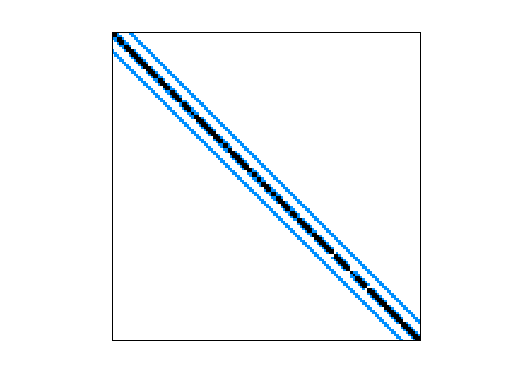
\includegraphics[width=\linewidth]{spmv_matrices/saylr4.png} & 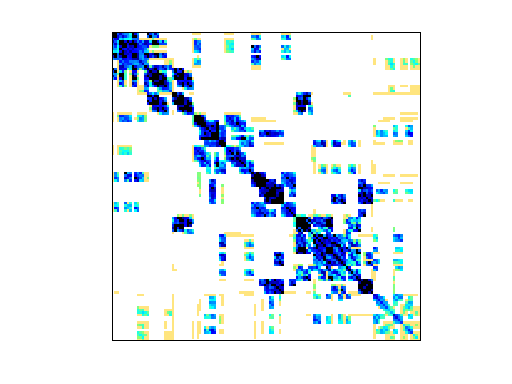
\includegraphics[width=\linewidth]{spmv_matrices/heart3.png} & 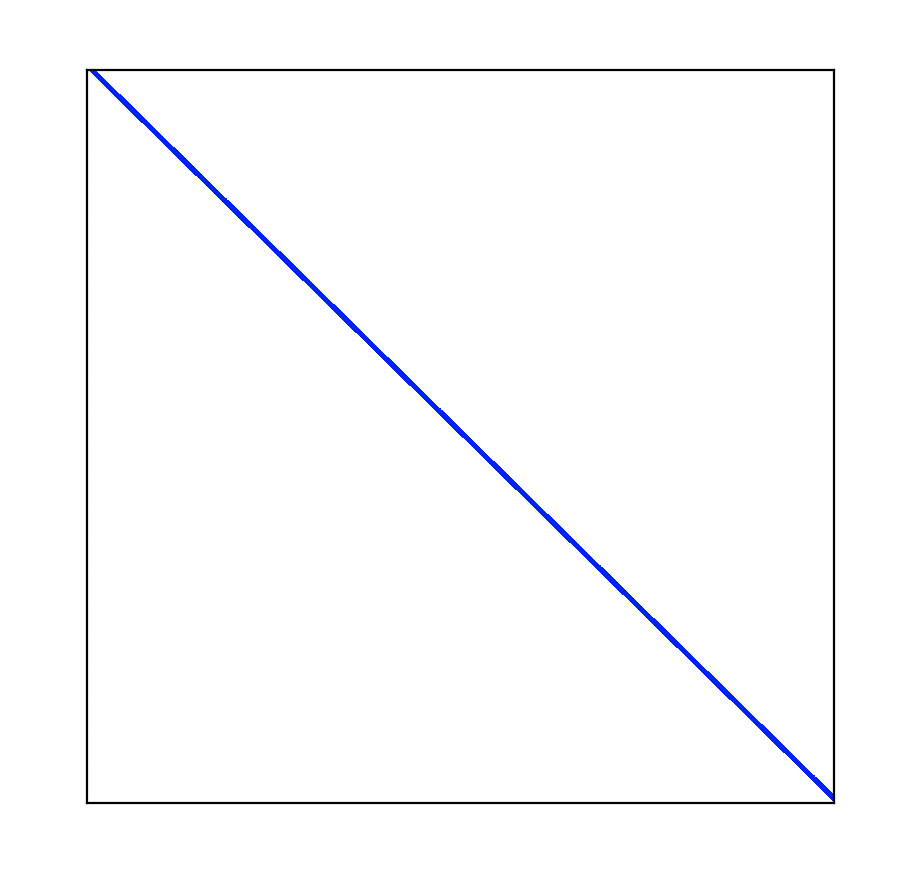
\includegraphics[width=\linewidth]{spmv_matrices/toeplitz_large_band.png} & 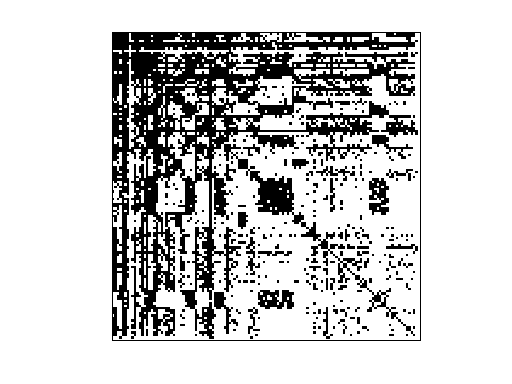
\includegraphics[width=\linewidth]{spmv_matrices/as-735.png} \\
      \hline 
      \textbf{Group / Name} & HB/saylr4 & Norris/heart3 & large\_band & SNAP/as-735 \\
      \hline
      \textbf{Dimensions} & 3,564 x 3,564 (22,316) & 2,339 x 2,339 (680,341) & 10,000 x 10,000 (1,999,900) & 7,716 x 7,716 (26,467) \\
      \hline
      \textbf{Best Finch Format} & Symmetric SparseList & SparseVBL & SparseBand & Symmetric SparseList-Pattern \\
      \hline
  \end{tabular}
  \vspace{-8pt}
\end{table}

\section{Graph Algorithm Listings}\label{sec:graph_listings}

\subsection{Finch Breadth-First Search}
\begin{minted}{julia}
    function bfs_finch_kernel(edges, edgesT, source=5, alpha = 0.01)
    (n, m) = size(edges)
    edges = pattern!(edges)
    @assert n == m
    F = Tensor(SparseByteMap(Pattern()), n)
    _F = Tensor(SparseByteMap(Pattern()), n)
    @finch F[source] = true
    F_nnz = 1 
    V = Tensor(Dense(Element(false)), n)
    @finch V[source] = true
    P = Tensor(Dense(Element(0)), n)
    @finch P[source] = source
    while F_nnz > 0 
        if F_nnz/m > alpha # pull
            p = ShortCircuitScalar{0}()
            _F .= false
            for k=_ 
                if !V[k]
                    p .= 0
                    for j=_ 
                        if F[follow(j)] && AT[j, k]
                            p[] <<choose(0)>>= j
                        end 
                    end 
                    if p[] != 0
                        _F[k] |= true
                        P[k] = p[] 
                    end 
                end 
            end
        else # push
            _F .= false
            for j=_, k=_ 
                if F[j] && A[k, j] && !(V[k])
                    _F[k] |= true
                    P[k] <<choose(0)>>= j
                end 
            end 
        end 
        c = Scalar(0)
        @finch begin
            for k=_ 
                let _f = _F[k]
                    V[k] |= _f
                    c[] += _f
                end 
            end 
        end 
        (F, _F) = (_F, F)
        F_nnz = c[] 
    end 
    return P
end
\end{minted}
\subsection{GraphBLAS Breadth-First Search}
\begin{minted}{c}
//------------------------------------------------------------------------------
// LAGr_BreadthFirstSearch:  breadth-first search dispatch
//------------------------------------------------------------------------------

// LAGraph, (c) 2019-2022 by The LAGraph Contributors, All Rights Reserved.
// SPDX-License-Identifier: BSD-2-Clause
//
// For additional details (including references to third party source code and
// other files) see the LICENSE file or contact permission@sei.cmu.edu. See
// Contributors.txt for a full list of contributors. Created, in part, with
// funding and support from the U.S. Government (see Acknowledgments.txt file).
// DM22-0790

// Contributed by Scott McMillan, SEI Carnegie Mellon University

//------------------------------------------------------------------------------

// Breadth-first-search via push/pull method if using SuiteSparse:GraphBLAS
// and its GxB extensions, or a push-only method otherwise.  The former is
// much faster.

// This is an Advanced algorithm.  SuiteSparse can use a push/pull method if
// G->AT and G->out_degree are provided.  G->AT is not required if G is
// undirected.  The vanilla method is always push-only.

#include "LG_alg_internal.h"

int LAGr_BreadthFirstSearch
(
    // output:
    GrB_Vector *level,
    GrB_Vector *parent,
    // input:
    const LAGraph_Graph G,
    GrB_Index src,
    char *msg
)
{

#if LAGRAPH_SUITESPARSE
    return LG_BreadthFirstSearch_SSGrB   (level, parent, G, src, msg) ;
#else
    return LG_BreadthFirstSearch_vanilla (level, parent, G, src, msg) ;
#endif
}

//------------------------------------------------------------------------------
// LG_BreadthFirstSearch_SSGrB:  BFS using Suitesparse extensions
//------------------------------------------------------------------------------

// LAGraph, (c) 2019-2022 by The LAGraph Contributors, All Rights Reserved.
// SPDX-License-Identifier: BSD-2-Clause
//
// For additional details (including references to third party source code and
// other files) see the LICENSE file or contact permission@sei.cmu.edu. See
// Contributors.txt for a full list of contributors. Created, in part, with
// funding and support from the U.S. Government (see Acknowledgments.txt file).
// DM22-0790

// Contributed by Timothy A. Davis, Texas A&M University

//------------------------------------------------------------------------------

// This is an Advanced algorithm.  G->AT and G->out_degree are required for
// this method to use push-pull optimization.  If not provided, this method
// defaults to a push-only algorithm, which can be slower.  This is not
// user-callable (see LAGr_BreadthFirstSearch instead).  G->AT and
// G->out_degree are not computed if not present.

// References:
//
// Carl Yang, Aydin Buluc, and John D. Owens. 2018. Implementing Push-Pull
// Efficiently in GraphBLAS. In Proceedings of the 47th International
// Conference on Parallel Processing (ICPP 2018). ACM, New York, NY, USA,
// Article 89, 11 pages. DOI: https://doi.org/10.1145/3225058.3225122
//
// Scott Beamer, Krste Asanovic and David A. Patterson, The GAP Benchmark
// Suite, http://arxiv.org/abs/1508.03619, 2015.  http://gap.cs.berkeley.edu/

// revised by Tim Davis (davis@tamu.edu), Texas A&M University

#define LG_FREE_WORK        \
{                           \
    GrB_free (&w) ;         \
    GrB_free (&q) ;         \
}

#define LG_FREE_ALL         \
{                           \
    LG_FREE_WORK ;          \
    GrB_free (&pi) ;        \
    GrB_free (&v) ;         \
}

#include "LG_internal.h"

int LG_BreadthFirstSearch_SSGrB
(
    GrB_Vector *level,
    GrB_Vector *parent,
    const LAGraph_Graph G,
    GrB_Index src,
    char *msg
)
{

    //--------------------------------------------------------------------------
    // check inputs
    //--------------------------------------------------------------------------

    LG_CLEAR_MSG ;
    GrB_Vector q = NULL ;           // the current frontier
    GrB_Vector w = NULL ;           // to compute work remaining
    GrB_Vector pi = NULL ;          // parent vector
    GrB_Vector v = NULL ;           // level vector

#if !LAGRAPH_SUITESPARSE
    LG_ASSERT (false, GrB_NOT_IMPLEMENTED) ;
#else

    bool compute_level  = (level != NULL) ;
    bool compute_parent = (parent != NULL) ;
    if (compute_level ) (*level ) = NULL ;
    if (compute_parent) (*parent) = NULL ;
    LG_ASSERT_MSG (compute_level || compute_parent, GrB_NULL_POINTER,
        "either level or parent must be non-NULL") ;

    LG_TRY (LAGraph_CheckGraph (G, msg)) ;

    //--------------------------------------------------------------------------
    // get the problem size and cached properties
    //--------------------------------------------------------------------------

    GrB_Matrix A = G->A ;

    GrB_Index n, nvals ;
    GRB_TRY (GrB_Matrix_nrows (&n, A)) ;
    LG_ASSERT_MSG (src < n, GrB_INVALID_INDEX, "invalid source node") ;

    GRB_TRY (GrB_Matrix_nvals (&nvals, A)) ;

    GrB_Matrix AT = NULL ;
    GrB_Vector Degree = G->out_degree ;
    if (G->kind == LAGraph_ADJACENCY_UNDIRECTED ||
       (G->kind == LAGraph_ADJACENCY_DIRECTED &&
        G->is_symmetric_structure == LAGraph_TRUE))
    {
        // AT and A have the same structure and can be used in both directions
        AT = G->A ;
    }
    else
    {
        // AT = A' is different from A.  If G->AT is NULL, then a push-only
        // method is used.
        AT = G->AT ;
    }

    // direction-optimization requires G->AT (if G is directed) and
    // G->out_degree (for both undirected and directed cases)
    bool push_pull = (Degree != NULL && AT != NULL) ;

    // determine the semiring type
    GrB_Type int_type = (n > INT32_MAX) ? GrB_INT64 : GrB_INT32 ;
    GrB_Semiring semiring ;

    if (compute_parent)
    {
        // use the ANY_SECONDI_INT* semiring: either 32 or 64-bit depending on
        // the # of nodes in the graph.
        semiring = (n > INT32_MAX) ?
            GxB_ANY_SECONDI_INT64 : GxB_ANY_SECONDI_INT32 ;

        // create the parent vector.  pi(i) is the parent id of node i
        GRB_TRY (GrB_Vector_new (&pi, int_type, n)) ;
        GRB_TRY (GxB_set (pi, GxB_SPARSITY_CONTROL, GxB_BITMAP + GxB_FULL)) ;
        // pi (src) = src denotes the root of the BFS tree
        GRB_TRY (GrB_Vector_setElement (pi, src, src)) ;

        // create a sparse integer vector q, and set q(src) = src
        GRB_TRY (GrB_Vector_new (&q, int_type, n)) ;
        GRB_TRY (GrB_Vector_setElement (q, src, src)) ;
    }
    else
    {
        // only the level is needed, use the LAGraph_any_one_bool semiring
        semiring = LAGraph_any_one_bool ;

        // create a sparse boolean vector q, and set q(src) = true
        GRB_TRY (GrB_Vector_new (&q, GrB_BOOL, n)) ;
        GRB_TRY (GrB_Vector_setElement (q, true, src)) ;
    }

    if (compute_level)
    {
        // create the level vector. v(i) is the level of node i
        // v (src) = 0 denotes the source node
        GRB_TRY (GrB_Vector_new (&v, int_type, n)) ;
        GRB_TRY (GxB_set (v, GxB_SPARSITY_CONTROL, GxB_BITMAP + GxB_FULL)) ;
        GRB_TRY (GrB_Vector_setElement (v, 0, src)) ;
    }

    // workspace for computing work remaining
    GRB_TRY (GrB_Vector_new (&w, GrB_INT64, n)) ;

    GrB_Index nq = 1 ;          // number of nodes in the current level
    double alpha = 8.0 ;
    double beta1 = 8.0 ;
    double beta2 = 512.0 ;
    int64_t n_over_beta1 = (int64_t) (((double) n) / beta1) ;
    int64_t n_over_beta2 = (int64_t) (((double) n) / beta2) ;

    //--------------------------------------------------------------------------
    // BFS traversal and label the nodes
    //--------------------------------------------------------------------------

    bool do_push = true ;       // start with push
    GrB_Index last_nq = 0 ;
    int64_t edges_unexplored = nvals ;
    bool any_pull = false ;     // true if any pull phase has been done

    // {!mask} is the set of unvisited nodes
    GrB_Vector mask = (compute_parent) ? pi : v ;

    for (int64_t nvisited = 1, k = 1 ; nvisited < n ; nvisited += nq, k++)
    {

        //----------------------------------------------------------------------
        // select push vs pull
        //----------------------------------------------------------------------

        if (push_pull)
        {
            if (do_push)
            {
                // check for switch from push to pull
                bool growing = nq > last_nq ;
                bool switch_to_pull = false ;
                if (edges_unexplored < n)
                {
                    // very little of the graph is left; disable the pull
                    push_pull = false ;
                }
                else if (any_pull)
                {
                    // once any pull phase has been done, the # of edges in the
                    // frontier has no longer been tracked.  But now the BFS
                    // has switched back to push, and we're checking for yet
                    // another switch to pull.  This switch is unlikely, so
                    // just keep track of the size of the frontier, and switch
                    // if it starts growing again and is getting big.
                    switch_to_pull = (growing && nq > n_over_beta1) ;
                }
                else
                {
                    // update the # of unexplored edges
                    // w<q>=Degree
                    // w(i) = outdegree of node i if node i is in the queue
                    GRB_TRY (GrB_assign (w, q, NULL, Degree, GrB_ALL, n,
                        GrB_DESC_RS)) ;
                    // edges_in_frontier = sum (w) = # of edges incident on all
                    // nodes in the current frontier
                    int64_t edges_in_frontier = 0 ;
                    GRB_TRY (GrB_reduce (&edges_in_frontier, NULL,
                        GrB_PLUS_MONOID_INT64, w, NULL)) ;
                    edges_unexplored -= edges_in_frontier ;
                    switch_to_pull = growing &&
                        (edges_in_frontier > (edges_unexplored / alpha)) ;
                }
                if (switch_to_pull)
                {
                    // switch from push to pull
                    do_push = false ;
                }
            }
            else
            {
                // check for switch from pull to push
                bool shrinking = nq < last_nq ;
                if (shrinking && (nq <= n_over_beta2))
                {
                    // switch from pull to push
                    do_push = true ;
                }
            }
            any_pull = any_pull || (!do_push) ;
        }

        //----------------------------------------------------------------------
        // q = kth level of the BFS
        //----------------------------------------------------------------------

        int sparsity = do_push ? GxB_SPARSE : GxB_BITMAP ;
        GRB_TRY (GxB_set (q, GxB_SPARSITY_CONTROL, sparsity)) ;

        // mask is pi if computing parent, v if computing just level
        if (do_push)
        {
            // push (saxpy-based vxm):  q'{!mask} = q'*A
            GRB_TRY (GrB_vxm (q, mask, NULL, semiring, q, A, GrB_DESC_RSC)) ;
        }
        else
        {
            // pull (dot-product-based mxv):  q{!mask} = AT*q
            GRB_TRY (GrB_mxv (q, mask, NULL, semiring, AT, q, GrB_DESC_RSC)) ;
        }

        //----------------------------------------------------------------------
        // done if q is empty
        //----------------------------------------------------------------------

        last_nq = nq ;
        GRB_TRY (GrB_Vector_nvals (&nq, q)) ;
        if (nq == 0)
        {
            break ;
        }

        //----------------------------------------------------------------------
        // assign parents/levels
        //----------------------------------------------------------------------

        if (compute_parent)
        {
            // q(i) currently contains the parent id of node i in tree.
            // pi{q} = q
            GRB_TRY (GrB_assign (pi, q, NULL, q, GrB_ALL, n, GrB_DESC_S)) ;
        }
        if (compute_level)
        {
            // v{q} = k, the kth level of the BFS
            GRB_TRY (GrB_assign (v, q, NULL, k, GrB_ALL, n, GrB_DESC_S)) ;
        }
    }

    //--------------------------------------------------------------------------
    // free workspace and return result
    //--------------------------------------------------------------------------

    if (compute_parent) (*parent) = pi ;
    if (compute_level ) (*level ) = v ;
    LG_FREE_WORK ;
    return (GrB_SUCCESS) ;
#endif
}
\end{minted}
\subsection{Finch Bellman-Ford}
\begin{minted}{julia}
function bellmanford_finch_kernel(edges, source=1)
    (n, m) = size(edges)
    @assert n == m
    dists_prev = Tensor(Dense(Element(Inf)), n)
    dists_prev[source] = 0 
    dists = Tensor(Dense(Element(Inf)), n)
    active_prev = Tensor(SparseByteMap(Pattern()), n)
    active_prev[source] = true
    active = Tensor(SparseByteMap(Pattern()), n)
    parents = Tensor(Dense(Element(0)), n)
    for iter = 1:n  
        @finch begin
            for j=_ 
                if active_prev[j]
                    dists[j] <<min>>= dists_prev[j]
                end 
            end 
        end 
        @finch begin
            active .= false
            for j = _ 
                if active_prev[j]
                    for i = _ 
                        let d = dists_prev[j] + edges[i, j]
                            dists[i] <<min>>= d
                            active[i] |= d < dists_prev[i]
                        end 
                    end 
                end 
            end 
        end 
        if countstored(active) == 0
            break
        end 
        dists_prev, dists = dists, dists_prev
        active_prev, active = active, active_prev
    end 
    @finch begin
        for j = _ 
            for i = _ 
                let d = edges[i, j]
                    if d < Inf && dists[j] + d <= dists[i]
                        parents[i] <<choose(0)>>= j
                    end 
                end 
            end 
        end 
    end 
    return (dists=dists, parents=parents)
end
\end{minted}

\subsection{GraphBLAS Bellman-Ford}
\begin{minted}{c}
//------------------------------------------------------------------------------
// LAGraph_BF_full1a.c: Bellman-Ford single-source shortest paths, returns tree,
// while diagonal of input matrix A needs not to be explicit 0
//------------------------------------------------------------------------------

// LAGraph, (c) 2019-2022 by The LAGraph Contributors, All Rights Reserved.
// SPDX-License-Identifier: BSD-2-Clause
//
// For additional details (including references to third party source code and
// other files) see the LICENSE file or contact permission@sei.cmu.edu. See
// Contributors.txt for a full list of contributors. Created, in part, with
// funding and support from the U.S. Government (see Acknowledgments.txt file).
// DM22-0790

// Contributed by Jinhao Chen and Timothy A. Davis, Texas A&M University

//------------------------------------------------------------------------------

// This is the fastest variant that computes both the parent & the path length.

// LAGraph_BF_full1a: Bellman-Ford single source shortest paths, returning both
// the path lengths and the shortest-path tree.

// LAGraph_BF_full performs a Bellman-Ford to find out shortest path, parent
// nodes along the path and the hops (number of edges) in the path from given
// source vertex s in the range of [0, n) on graph given as matrix A with size
// n*n. The sparse matrix A has entry A(i, j) if there is an edge from vertex i
// to vertex j with weight w, then A(i, j) = w.

// LAGraph_BF_full1a returns GrB_SUCCESS if it succeeds.  In this case, there
// are no negative-weight cycles in the graph, and d, pi, and h are returned.
// The vector d has d(k) as the shortest distance from s to k. pi(k) = p+1,
// where p is the parent node of k-th node in the shortest path. In particular,
// pi(s) = 0. h(k) = hop(s, k), the number of edges from s to k in the shortest
// path.

// If the graph has a negative-weight cycle, GrB_NO_VALUE is returned, and the
// GrB_Vectors d(k), pi(k) and h(k)  (i.e., *pd_output, *ppi_output and
// *ph_output respectively) will be NULL when negative-weight cycle detected.

// Otherwise, other errors such as GrB_OUT_OF_MEMORY, GrB_INVALID_OBJECT, and
// so on, can be returned, if these errors are found by the underlying
// GrB_* functions.

//------------------------------------------------------------------------------

#define LG_FREE_WORK                   \
{                                      \
    GrB_free(&d);                      \
    GrB_free(&dmasked);                \
    GrB_free(&dless);                  \
    GrB_free(&Atmp);                   \
    GrB_free(&BF_Tuple3);              \
    GrB_free(&BF_lMIN_Tuple3);         \
    GrB_free(&BF_PLUSrhs_Tuple3);      \
    GrB_free(&BF_LT_Tuple3);           \
    GrB_free(&BF_lMIN_Tuple3_Monoid);  \
    GrB_free(&BF_lMIN_PLUSrhs_Tuple3); \
    LAGraph_Free ((void**)&I, NULL);   \
    LAGraph_Free ((void**)&J, NULL);   \
    LAGraph_Free ((void**)&w, NULL);   \
    LAGraph_Free ((void**)&W, NULL);   \
    LAGraph_Free ((void**)&h, NULL);   \
    LAGraph_Free ((void**)&pi, NULL);  \
}

#define LG_FREE_ALL                    \
{                                      \
    LG_FREE_WORK ;                     \
    GrB_free (pd_output);              \
    GrB_free (ppi_output);             \
    GrB_free (ph_output);              \
}

#include <LAGraph.h>
#include <LAGraphX.h>
#include <LG_internal.h>  // from src/utility

typedef void (*LAGraph_binary_function) (void *, const void *, const void *) ;

//------------------------------------------------------------------------------
// data type for each entry of the adjacent matrix A and "distance" vector d;
// <INFINITY,INFINITY,INFINITY> corresponds to nonexistence of a path, and
// the value  <0, 0, NULL> corresponds to a path from a vertex to itself
//------------------------------------------------------------------------------

typedef struct
{
    double w;    // w  corresponds to a path weight.
    GrB_Index h; // h  corresponds to a path size or number of hops.
    GrB_Index pi;// pi corresponds to the penultimate vertex along a path.
                 // vertex indexed as 1, 2, 3, ... , V, and pi = 0 (as nil)
                 // for u=v, and pi = UINT64_MAX (as inf) for (u,v) not in E
}
BF_Tuple3_struct;

//------------------------------------------------------------------------------
// binary functions, z=f(x,y), where Tuple3xTuple3 -> Tuple3
//------------------------------------------------------------------------------

void BF_lMIN3
(
    BF_Tuple3_struct *z,
    const BF_Tuple3_struct *x,
    const BF_Tuple3_struct *y
)
{
    if (x->w < y->w
        || (x->w == y->w && x->h < y->h)
        || (x->w == y->w && x->h == y->h && x->pi < y->pi))
    {
        if (z != x) { *z = *x; }
    }
    else
    {
        *z = *y;
    }
}

void BF_PLUSrhs3
(
    BF_Tuple3_struct *z,
    const BF_Tuple3_struct *x,
    const BF_Tuple3_struct *y
)
{
    z->w = x->w + y->w ;
    z->h = x->h + y->h ;
    z->pi = (x->pi != UINT64_MAX && y->pi != 0) ?  y->pi : x->pi ;
}

void BF_LT3
(
    bool *z,
    const BF_Tuple3_struct *x,
    const BF_Tuple3_struct *y
)
{
    (*z) = (x->w < y->w
        || (x->w == y->w && x->h < y->h)
        || (x->w == y->w && x->h == y->h && x->pi < y->pi)) ;
}

// Given a n-by-n adjacency matrix A and a source vertex s.
// If there is no negative-weight cycle reachable from s, return the distances
// of shortest paths from s and parents along the paths as vector d. Otherwise,
// returns d=NULL if there is a negtive-weight cycle.
// pd_output is pointer to a GrB_Vector, where the i-th entry is d(s,i), the
//   sum of edges length in the shortest path
// ppi_output is pointer to a GrB_Vector, where the i-th entry is pi(i), the
//   parent of i-th vertex in the shortest path
// ph_output is pointer to a GrB_Vector, where the i-th entry is h(s,i), the
//   number of edges from s to i in the shortest path
// A has weights on corresponding entries of edges
// s is given index for source vertex
GrB_Info LAGraph_BF_full1a
(
    GrB_Vector *pd_output,      //the pointer to the vector of distance
    GrB_Vector *ppi_output,     //the pointer to the vector of parent
    GrB_Vector *ph_output,      //the pointer to the vector of hops
    const GrB_Matrix A,         //matrix for the graph
    const GrB_Index s           //given index of the source
)
{
    GrB_Info info;
    char *msg = NULL ;
    // tmp vector to store distance vector after n (i.e., V) loops
    GrB_Vector d = NULL, dmasked = NULL, dless = NULL;
    GrB_Matrix Atmp = NULL;
    GrB_Type BF_Tuple3;

    GrB_BinaryOp BF_lMIN_Tuple3;
    GrB_BinaryOp BF_PLUSrhs_Tuple3;
    GrB_BinaryOp BF_LT_Tuple3;

    GrB_Monoid BF_lMIN_Tuple3_Monoid;
    GrB_Semiring BF_lMIN_PLUSrhs_Tuple3;

    GrB_Index nrows, ncols, n, nz;  // n = # of row/col, nz = # of nnz in graph
    GrB_Index *I = NULL, *J = NULL; // for col/row indices of entries from A
    GrB_Index *h = NULL, *pi = NULL;
    double *w = NULL;
    BF_Tuple3_struct *W = NULL;

    if (pd_output  != NULL) *pd_output  = NULL;
    if (ppi_output != NULL) *ppi_output = NULL;
    if (ph_output  != NULL) *ph_output  = NULL;

    LG_ASSERT (A != NULL && pd_output != NULL &&
        ppi_output != NULL && ph_output != NULL, GrB_NULL_POINTER) ;

    GRB_TRY (GrB_Matrix_nrows (&nrows, A)) ;
    GRB_TRY (GrB_Matrix_ncols (&ncols, A)) ;
    GRB_TRY (GrB_Matrix_nvals (&nz, A));
    LG_ASSERT_MSG (nrows == ncols, -1002, "A must be square") ;
    n = nrows;
    LG_ASSERT_MSG (s < n, GrB_INVALID_INDEX, "invalid source node") ;

    //--------------------------------------------------------------------------
    // create all GrB_Type GrB_BinaryOp GrB_Monoid and GrB_Semiring
    //--------------------------------------------------------------------------
    // GrB_Type
    GRB_TRY (GrB_Type_new(&BF_Tuple3, sizeof(BF_Tuple3_struct)));

    // GrB_BinaryOp
    GRB_TRY (GrB_BinaryOp_new(&BF_LT_Tuple3,
        (LAGraph_binary_function) (&BF_LT3), GrB_BOOL, BF_Tuple3, BF_Tuple3));
    GRB_TRY (GrB_BinaryOp_new(&BF_lMIN_Tuple3,
        (LAGraph_binary_function) (&BF_lMIN3), BF_Tuple3, BF_Tuple3,BF_Tuple3));
    GRB_TRY (GrB_BinaryOp_new(&BF_PLUSrhs_Tuple3,
        (LAGraph_binary_function)(&BF_PLUSrhs3),
        BF_Tuple3, BF_Tuple3, BF_Tuple3));

    // GrB_Monoid
    BF_Tuple3_struct BF_identity = (BF_Tuple3_struct) { .w = INFINITY,
        .h = UINT64_MAX, .pi = UINT64_MAX };
    GRB_TRY (GrB_Monoid_new_UDT(&BF_lMIN_Tuple3_Monoid, BF_lMIN_Tuple3,
        &BF_identity));

    //GrB_Semiring
    GRB_TRY (GrB_Semiring_new(&BF_lMIN_PLUSrhs_Tuple3,
        BF_lMIN_Tuple3_Monoid, BF_PLUSrhs_Tuple3));

    //--------------------------------------------------------------------------
    // allocate arrays used for tuplets
    //--------------------------------------------------------------------------
#if 1
    LAGRAPH_TRY (LAGraph_Malloc ((void **) &I, nz, sizeof(GrB_Index), msg)) ;
    LAGRAPH_TRY (LAGraph_Malloc ((void **) &J, nz, sizeof(GrB_Index), msg)) ;
    LAGRAPH_TRY (LAGraph_Malloc ((void **) &w, nz, sizeof(double), msg)) ;
    LAGRAPH_TRY (LAGraph_Malloc ((void **) &W, nz, sizeof(BF_Tuple3_struct),
        msg)) ;

    //--------------------------------------------------------------------------
    // create matrix Atmp based on A, while its entries become BF_Tuple3 type
    //--------------------------------------------------------------------------

    GRB_TRY (GrB_Matrix_extractTuples_FP64(I, J, w, &nz, A));
    int nthreads, nthreads_outer, nthreads_inner ;
    LG_TRY (LAGraph_GetNumThreads (&nthreads_outer, &nthreads_inner, msg)) ;
    nthreads = nthreads_outer * nthreads_inner ;
    printf ("nthreads %d\n", nthreads) ;
    int64_t k;
    #pragma omp parallel for num_threads(nthreads) schedule(static)
    for (k = 0; k < nz; k++)
    {
        W[k] = (BF_Tuple3_struct) { .w = w[k], .h = 1, .pi = I[k] + 1 };
    }
    GRB_TRY (GrB_Matrix_new(&Atmp, BF_Tuple3, n, n));
    GRB_TRY (GrB_Matrix_build_UDT(Atmp, I, J, W, nz, BF_lMIN_Tuple3));
    LAGraph_Free ((void**)&I, NULL);
    LAGraph_Free ((void**)&J, NULL);
    LAGraph_Free ((void**)&W, NULL);
    LAGraph_Free ((void**)&w, NULL);

#else

    todo: GraphBLAS could use a new kind of unary operator, not z=f(x), but

    [z,flag] = f (aij, i, j, k, nrows, ncols, nvals, etc, ...)
    flag: keep or discard.  Combines GrB_apply and GxB_select.

    builtins:
        f(...) =
            i, bool is true
            j, bool is true
            i+j*nrows, etc.
            k
            tril, triu (like GxB_select): return aij, and true/false boolean

        z=f(x,i).  x: double, z:tuple3, i:GrB_Index with the row index of x
        // z = (BF_Tuple3_struct) { .w = x, .h = 1, .pi = i + 1 };

    GrB_apply (Atmp, op, A, ...)

    in the BFS, this is used:
        op:  z = f ( .... ) = i
        to replace x(i) with i

#endif

    //--------------------------------------------------------------------------
    // create and initialize "distance" vector d, dmasked and dless
    //--------------------------------------------------------------------------
    GRB_TRY (GrB_Vector_new(&d, BF_Tuple3, n));
    // make d dense
    GRB_TRY (GrB_Vector_assign_UDT(d, NULL, NULL, (void*)&BF_identity,
        GrB_ALL, n, NULL));
    // initial distance from s to itself
    BF_Tuple3_struct d0 = (BF_Tuple3_struct) { .w = 0, .h = 0, .pi = 0 };
    GRB_TRY (GrB_Vector_setElement_UDT(d, &d0, s));

    // creat dmasked as a sparse vector with only one entry at s
    GRB_TRY (GrB_Vector_new(&dmasked, BF_Tuple3, n));
    GRB_TRY (GrB_Vector_setElement_UDT(dmasked, &d0, s));

    // create dless
    GRB_TRY (GrB_Vector_new(&dless, GrB_BOOL, n));

    //--------------------------------------------------------------------------
    // start the Bellman Ford process
    //--------------------------------------------------------------------------
    bool any_dless= true;      // if there is any newly found shortest path
    int64_t iter = 0;          // number of iterations

    // terminate when no new path is found or more than V-1 loops
    while (any_dless && iter < n - 1)
    {
        // execute semiring on dmasked and A, and save the result to dmasked
        GRB_TRY (GrB_vxm(dmasked, GrB_NULL, GrB_NULL,
            BF_lMIN_PLUSrhs_Tuple3, dmasked, Atmp, GrB_NULL));

        // dless = d .< dtmp
        GRB_TRY (GrB_eWiseMult(dless, NULL, NULL, BF_LT_Tuple3, dmasked, d,
            NULL));

        // if there is no entry with smaller distance then all shortest paths
        // are found
        GRB_TRY (GrB_reduce (&any_dless, NULL, GrB_LOR_MONOID_BOOL, dless,
            NULL)) ;
        if(any_dless)
        {
            // update all entries with smaller distances
            //GRB_TRY (GrB_apply(d, dless, NULL, BF_Identity_Tuple3,
            //    dmasked, NULL));
            GRB_TRY (GrB_assign(d, dless, NULL, dmasked, GrB_ALL, n, NULL));

            // only use entries that were just updated
            //GRB_TRY (GrB_Vector_clear(dmasked));
            //GRB_TRY (GrB_apply(dmasked, dless, NULL, BF_Identity_Tuple3,
            //    d, NULL));
            //try:
            GRB_TRY (GrB_assign(dmasked, dless, NULL, d, GrB_ALL, n, GrB_DESC_R));
        }
        iter ++;
    }

    // check for negative-weight cycle only when there was a new path in the
    // last loop, otherwise, there can't be a negative-weight cycle.
    if (any_dless)
    {
        // execute semiring again to check for negative-weight cycle
        GRB_TRY (GrB_vxm(dmasked, GrB_NULL, GrB_NULL,
            BF_lMIN_PLUSrhs_Tuple3, dmasked, Atmp, GrB_NULL));

        // dless = d .< dtmp
        GRB_TRY (GrB_eWiseMult(dless, NULL, NULL, BF_LT_Tuple3, dmasked, d,
            NULL));

        // if there is no entry with smaller distance then all shortest paths
        // are found
        GRB_TRY (GrB_reduce (&any_dless, NULL, GrB_LOR_MONOID_BOOL, dless,
            NULL)) ;
        if(any_dless)
        {
            // printf("A negative-weight cycle found. \n");
            LG_FREE_ALL;
            return (GrB_NO_VALUE) ;
        }
    }

    //--------------------------------------------------------------------------
    // extract tuple from "distance" vector d and create GrB_Vectors for output
    //--------------------------------------------------------------------------

    LAGRAPH_TRY (LAGraph_Malloc ((void **) &I, n, sizeof(GrB_Index), msg)) ;
    LAGRAPH_TRY (LAGraph_Malloc ((void **) &W, n, sizeof(BF_Tuple3_struct),
        msg)) ;
    LAGRAPH_TRY (LAGraph_Malloc ((void **) &w, n, sizeof(double), msg)) ;
    LAGRAPH_TRY (LAGraph_Malloc ((void **) &h, n, sizeof(GrB_Index), msg)) ;
    LAGRAPH_TRY (LAGraph_Malloc ((void **) &pi, n, sizeof(GrB_Index), msg)) ;

    // todo: create 3 unary ops, and use GrB_apply?

    GRB_TRY (GrB_Vector_extractTuples_UDT (I, (void *) W, &n, d));

    for (k = 0; k < n; k++)
    {
        w [k] = W[k].w ;
        h [k] = W[k].h ;
        pi[k] = W[k].pi;
    }
    GRB_TRY (GrB_Vector_new(pd_output,  GrB_FP64,   n));
    GRB_TRY (GrB_Vector_new(ppi_output, GrB_UINT64, n));
    GRB_TRY (GrB_Vector_new(ph_output,  GrB_UINT64, n));
    GRB_TRY (GrB_Vector_build (*pd_output , I, w , n, GrB_MIN_FP64  ));
    GRB_TRY (GrB_Vector_build (*ppi_output, I, pi, n, GrB_MIN_UINT64));
    GRB_TRY (GrB_Vector_build (*ph_output , I, h , n, GrB_MIN_UINT64));
    LG_FREE_WORK;
    return (GrB_SUCCESS) ;
}

\end{minted}

\section{Mask Images}
We interpreted the following images from ``Digital Image Processing'' \cite{gonzalez_digital_2006} as masks:

\textbf{FigP1012.png}


\includegraphics[scale=0.20]{{./dip3e\_masks/FigP1012.png}}


\textbf{Fig1008\_a\_\_step edge\_.png}

\includegraphics[scale=0.20]{{./dip3e\_masks/Fig1008\_a\_\_step edge\_.png}}


\textbf{FigP0905\_d\_.png}

\includegraphics[scale=0.20]{{./dip3e\_masks/FigP0905\_d\_.png}}


\textbf{FigP0528\_c\_\_doughnut\_.png}

\includegraphics[scale=0.20]{{./dip3e\_masks/FigP0528\_c\_\_doughnut\_.png}}


\textbf{FigP0616\_b\_.png}

\includegraphics[scale=0.20]{{./dip3e\_masks/FigP0616\_b\_.png}}


\textbf{Fig0114\_c\_\_bottles\_.png}

\includegraphics[scale=0.20]{{./dip3e\_masks/Fig0114\_c\_\_bottles\_.png}}


\textbf{FigP0616\_c\_.png}

\includegraphics[scale=0.20]{{./dip3e\_masks/FigP0616\_c\_.png}}


\textbf{FigP0433\_b\_.png}

\includegraphics[scale=0.20]{{./dip3e\_masks/FigP0433\_b\_.png}}


\textbf{Figp0917.png}

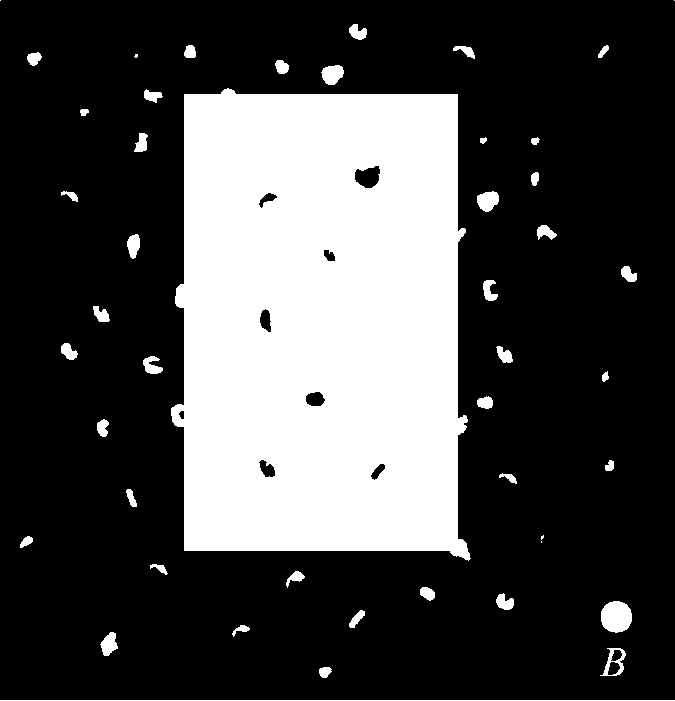
\includegraphics[scale=0.20]{{./dip3e\_masks/Figp0917.png}}


\textbf{FigP0905\_b\_.png}

\includegraphics[scale=0.20]{{./dip3e\_masks/FigP0905\_b\_.png}}


\textbf{Fig1059\_c\_\_NegADI\_.png}

\includegraphics[scale=0.20]{{./dip3e\_masks/Fig1059\_c\_\_NegADI\_.png}}


\textbf{Fig1111\_a\_\_triangle\_.png}

\includegraphics[scale=0.20]{{./dip3e\_masks/Fig1111\_a\_\_triangle\_.png}}


\textbf{Fig1111\_b\_\_square\_.png}

\includegraphics[scale=0.20]{{./dip3e\_masks/Fig1111\_b\_\_square\_.png}}


\textbf{FigP0905\_top\_.png}

\includegraphics[scale=0.20]{{./dip3e\_masks/FigP0905\_top\_.png}}


\textbf{FigP1110.png}


\includegraphics[scale=0.20]{{./dip3e\_masks/FigP1110.png}}


\textbf{Fig0533\_a\_\_circle\_.png}

\includegraphics[scale=0.20]{{./dip3e\_masks/Fig0533\_a\_\_circle\_.png}}


\textbf{FigP0917\_noisy\_rectangle\_.png}

\includegraphics[scale=0.20]{{./dip3e\_masks/FigP0917\_noisy\_rectangle\_.png}}


\textbf{Fig0230\_b\_\_dental\_xray\_mask\_.png}

\includegraphics[scale=0.20]{{./dip3e\_masks/Fig0230\_b\_\_dental\_xray\_mask\_.png}}


\textbf{FigP0528\_b\_\_two\_dots\_.png}

\includegraphics[scale=0.20]{{./dip3e\_masks/FigP0528\_b\_\_two\_dots\_.png}}


\textbf{Fig1059\_a\_\_AbsADI\_.png}

\includegraphics[scale=0.20]{{./dip3e\_masks/Fig1059\_a\_\_AbsADI\_.png}}


\textbf{Fig1059\_b\_\_PosADI\_.png}

\includegraphics[scale=0.20]{{./dip3e\_masks/Fig1059\_b\_\_PosADI\_.png}}


\textbf{Fig0539\_c\_\_shepp-logan\_phantom\_.png}

\includegraphics[scale=0.20]{{./dip3e\_masks/Fig0539\_c\_\_shepp-logan\_phantom\_.png}}


\textbf{FigP0905\_c\_.png}

\includegraphics[scale=0.20]{{./dip3e\_masks/FigP0905\_c\_.png}}


\textbf{Fig1043\_a\_\_yeast\_USC\_.png}

\includegraphics[scale=0.20]{{./dip3e\_masks/Fig1043\_a\_\_yeast\_USC\_.png}}


\textbf{FigP0905\_U\_.png}

\includegraphics[scale=0.20]{{./dip3e\_masks/FigP0905\_U\_.png}}


\textbf{Fig0524\_b\_\_blurred-impulse\_.png}

\includegraphics[scale=0.20]{{./dip3e\_masks/Fig0524\_b\_\_blurred-impulse\_.png}}


\textbf{Fig0424\_a\_\_rectangle\_.png}

\includegraphics[scale=0.20]{{./dip3e\_masks/Fig0424\_a\_\_rectangle\_.png}}


\textbf{Fig1008\_c\_\_roof\_edge\_.png}

\includegraphics[scale=0.20]{{./dip3e\_masks/Fig1008\_c\_\_roof\_edge\_.png}}


\textbf{Fig0539\_a\_\_vertical\_rectangle\_.png}

\includegraphics[scale=0.20]{{./dip3e\_masks/Fig0539\_a\_\_vertical\_rectangle\_.png}}


\textbf{FigP0905\_a\_.png}

\includegraphics[scale=0.20]{{./dip3e\_masks/FigP0905\_a\_.png}}


\textbf{FigP0433\_a\_.png}

\includegraphics[scale=0.20]{{./dip3e\_masks/FigP0433\_a\_.png}}


\textbf{Fig0.15\_a\_\_translated\_rectangle\_.png}

\includegraphics[scale=0.20]{{./dip3e\_masks/Fig0425\_a\_\_translated\_rectangle\_.png}}


\textbf{FigP0918\_c\_.png}

\includegraphics[scale=0.20]{{./dip3e\_masks/FigP0918\_c\_.png}}


\textbf{Fig0524\_a\_\_impulse\_.png}

\includegraphics[scale=0.20]{{./dip3e\_masks/Fig0524\_a\_\_impulse\_.png}}


\textbf{Fig0236\_a\_\_letter\_T\_.png}

\includegraphics[scale=0.20]{{./dip3e\_masks/Fig0236\_a\_\_letter\_T\_.png}}


\textbf{Fig0503 \_original\_pattern\_.png}

\includegraphics[scale=0.20]{{./dip3e\_masks/Fig0503 \_original\_pattern\_.png}}


\textbf{FigP0501.png}

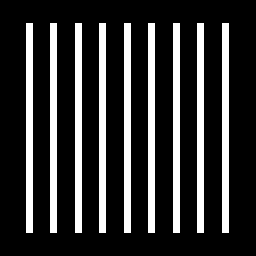
\includegraphics[scale=0.20]{{./dip3e\_masks/FigP0501.png}}


\textbf{Fig1218\_airplanes\_.png}

\includegraphics[scale=0.20]{{./dip3e\_masks/Fig1218\_airplanes\_.png}}


\textbf{Fig0534\_a\_\_ellipse\_and\_circle\_.png}

\includegraphics[scale=0.20]{{./dip3e\_masks/Fig0534\_a\_\_ellipse\_and\_circle\_.png}}


\textbf{FigP0616\_a\_.png}

\includegraphics[scale=0.20]{{./dip3e\_masks/FigP0616\_a\_.png}}


\textbf{FigP0918\_b\_.png}

\includegraphics[scale=0.20]{{./dip3e\_masks/FigP0918\_b\_.png}}


\textbf{FigP0528\_c\_.png}

\includegraphics[scale=0.20]{{./dip3e\_masks/FigP0528\_c\_.png}}


\textbf{FigP0528\_a\_\_single\_dot\_.png}

\includegraphics[scale=0.20]{{./dip3e\_masks/FigP0528\_a\_\_single\_dot\_.png}}


%%
%% The next two lines define the bibliography style to be used, and
%% the bibliography file.
\bibliographystyle{ACM-Reference-Format}
\bibliography{FinchOOPSLAWillow.bib}




\end{document}
\endinput